\documentclass[12pt]{article}

\usepackage[spanish]{babel}
\usepackage[none]{hyphenat}
\usepackage[left=1.5cm, right=1.5cm, top = 2cm, bottom=2.5cm]{geometry}
\usepackage{parskip}
\usepackage[export]{adjustbox}
\usepackage{enumitem}[shortlabels]
\usepackage{listings} 
\usepackage{color}
\usepackage{fancyhdr}
\usepackage{graphicx}
\usepackage{caption} 
% \usepackage{subcaption}
\usepackage{wrapfig}
% \usepackage{longtable}
% \usepackage{multirow, makecell}
% \usepackage{amsmath} 
\usepackage[hidelinks]{hyperref}
\usepackage{csquotes}
% \usepackage{tocloft}

\newcommand{\linejump}{\hfill \break}
\renewcommand{\thefootnote}{\fnsymbol{footnote}}
% \newcommand{\unit}[1]{\ensuremath{\, \mathrm{#1}}}

\definecolor{dkgreen}{rgb}{0,0.6,0}
\definecolor{gray}{rgb}{0.5,0.5,0.5}
\definecolor{mauve}{rgb}{0.58,0,0.82}
\lstset{
  language=Java,
  aboveskip=3mm,
  belowskip=3mm,
  showstringspaces=false,
  columns=flexible,
  basicstyle={\scriptsize\ttfamily},
  numbers=none,
  numberstyle=\tiny\color{gray},
  keywordstyle=\color{blue},
  commentstyle=\color{dkgreen},
  stringstyle=\color{mauve},
  breaklines=true,
  breakatwhitespace=true,
  tabsize=2
}

\sloppy
\setlength{\parindent}{0cm}
\setlength{\columnsep}{0.5cm}
\decimalpoint
\graphicspath{{img/}}

\hypersetup{colorlinks=true, urlcolor=blue, citecolor=blue}
\urlstyle{same}

\pagestyle{fancyplain}
\fancyhf{}
\fancyhead[L]{\scriptsize 
  Universidad Nacional Autónoma de México \\
  Programación Orientada a Objetos \\
  M.C. Leonardo Ledesma Dominguez
}
\fancyhead[R]{\thepage}


\begin{document}
  \begin{center}
    Acosta Porcayo Alan Omar 320206102 \\
    \linejump
    \LARGE \textbf{Tarea 7. Manejo de excepciones}
  \end{center}
  
  \linejump
  \begin{enumerate}
    \item Realice un cuadro sinóptico de excepciones y errores indicando:
    \begin{enumerate}[label=\alph*.]
      \item Excepciones
      \begin{enumerate}[label=\roman*.]
        \item Marcadas (Tiempo de compilación)
        \item No Marcadas (Tiempo de ejecución)
      \end{enumerate}
      \item Errores
      \begin{enumerate}[label=\roman*.]
        \item Sintácticos (Tiempo de compilación)
        \item Semánticos (Tiempo de ejecución)
      \end{enumerate}
    \end{enumerate}

    \begin{figure}[h!]
      \centering
      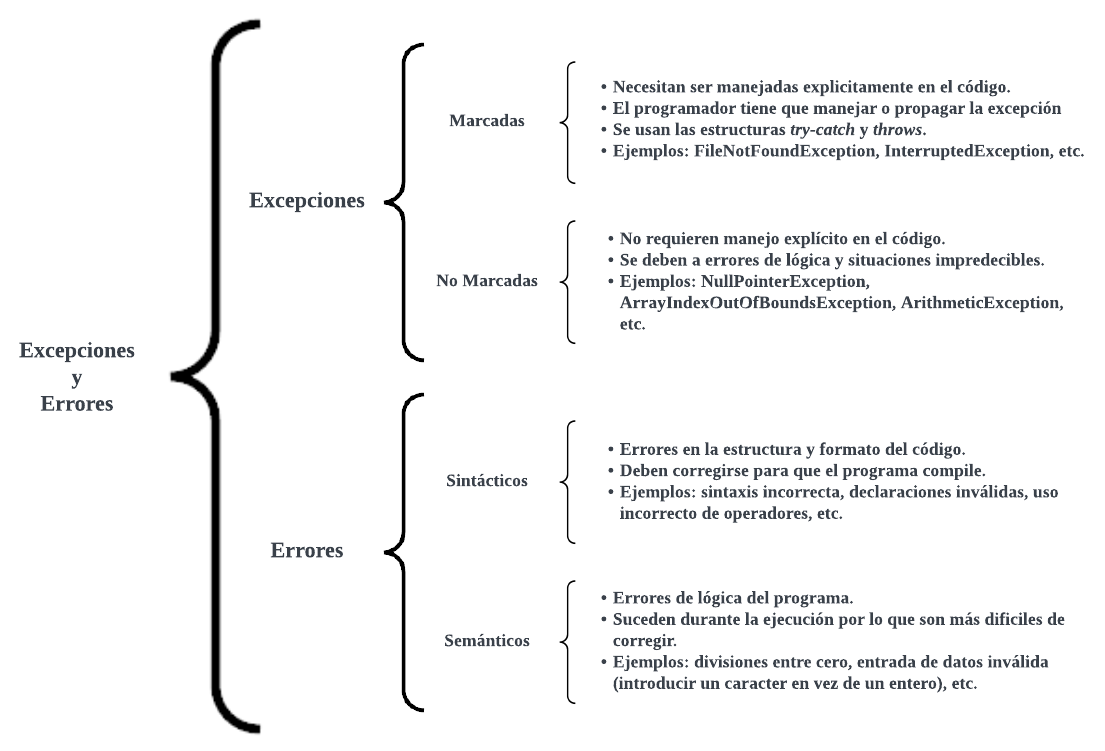
\includegraphics[width=0.9\textwidth]{sinoptico.png}
    \end{figure}

    \newpage
    \item Realice una tabla comparativa entre el uso de las palabras reservadas \textit{throw} y \textit{throws}.
    
    \begin{table}[h!]
      \centering
      \begin{tabular}{|p{0.45\textwidth}|p{0.45\textwidth}|}
        \hline
        \begin{center} \textbf{\textit{throw}} \end{center} & \begin{center} \textbf{\textit{throws}} \end{center} \\ \hline 
        Se utiliza para lanzar una excepción explícitamente en el código. & Se usa en la declaración de un método para indicar que en alguna parte del código puede ocurrir esa excepción. \\ \hline
        Solo se pueden propagar excepciones no marcadas. & Solo se pueden propagar excepciones marcadas. \\ \hline
        La palabra reservada \textit{throw} se usa dentro del cuerpo del método. & La palabra reservada \textit{throws} se usa en la declaración del método. \\ \hline
        Después de la palabra reservada \textit{throw} se debe especificar una instancia de la clase \textit{Throwable} o una subclase de esta. & Después de la palabra reservada \textit{throws} se debe especificar una clase que extienda de \textit{Throwable}. \\ \hline
        Se puede lanzar una excepción a la vez. & Se pueden lanzar varias excepciones a la vez. \\ \hline
      \end{tabular}
    \end{table}

    \item Realice un programa ocupando interfaces y clases abstractas implementando al menos una excepción usando:
    \begin{enumerate}[label=\alph*.]
      \item \textit{try catch} - operación no válida
      \item \textit{try catch resources} - Tarjeta de debido/crédito no válida
      \item \textit{throw} - excepción propia sin saldo suficiente
      \item \textit{throws} - NIP incorrecto
    \end{enumerate}
    El programa simula un ATM considere las clases Banco (interfaz), ATM (clase concreta) que implementa a Banco, Tarjeta (clase abstracta), Tarjeta de débito / crédito hereda de Tarjeta (clase concreta) y Cliente(clase concreta). Considere que las opciones del cliente pueden hacer retirar, abonar y consultar saldo, así como el ATM, de disminuir /aumentar saldo, verificar saldo, verificar NIP.


    \item Lea y haga un resumen del capitulo 2 del libro que el profesor compartió en classroom de Richard Warburton: “\textit{JAVA 8 Lambdas}”.
  \end{enumerate}

  \section*{Referencias}
  \textit{Difference between throw and throws in java - javatpoint}. (2021). www.javatpoint.com. \url{https://www.javatpoint.com/difference-between-throw-and-throws-in-java} \\

  Warburton, R. (2014). \textit{Java 8 lambdas: Functionnal Programming for the Masses}. Oreilly $\&$ Associates Incorporated.
\end{document}